%-----------------------------------------------------------------------------
%               Template for sigplanconf LaTeX Class
%
% Name:         sigplanconf-template.tex
%
% Purpose:      A template for sigplanconf.cls, which is a LaTeX 2e class
%               file for SIGPLAN conference proceedings.
%
% Guide:        Refer to "Author's Guide to the ACM SIGPLAN Class,"
%               sigplanconf-guide.pdf
%
% Author:       Paul C. Anagnostopoulos
%               Windfall Software
%               978 371-2316
%               paul@windfall.com
%
% Created:      15 February 2005
%-----------------------------------------------------------------------------
\documentclass[9pt,preprint,nocopyrightspace,computermodern]{sigplanconf} %% ,preprint,nocopyrightspace

% The following \documentclass options may be useful:

% preprint      Remove this option only once the paper is in final form.
% 10pt          To set in 10-point type instead of 9-point.
% 11pt          To set in 11-point type instead of 9-point.
% authoryear    To obtain author/year citation style instead of numeric.

\usepackage{graphicx, color, xcolor}
\usepackage{amsmath}
\usepackage{hyperref}
\usepackage{fontspec}
\setmonofont[Scale=MatchLowercase]{Courier}
\usepackage{epigraph}
\usepackage{pmboxdraw}
\usepackage{textcomp}
\usepackage{acronym}
\usepackage{float}
\usepackage{balance}
\usepackage{amssymb}

%% mine
\usepackage{mathpartir}
\usepackage{titlesec}
\usepackage{proof}
\usepackage{tabu}
\usepackage{array}
\usepackage{tikz}
\usepackage{caption}
\usetikzlibrary{matrix}
\usetikzlibrary{arrows}

%%%%-------------------------------------------------------------------------------------
%% Old format stuff

%% \documentclass[18pt,twocolumn] {article}

%% \usepackage{amssymb}
%% \usepackage{amsmath}
%% \usepackage{mathpartir}
%% \usepackage{titlesec}
%% \usepackage{proof}
%% \usepackage{tabu}
%% \usepackage{array}
%% \usepackage{tikz}
%% \usetikzlibrary{matrix}

%% \titlespacing\section{0pt}{12pt plus 4pt minus 2pt}{0pt plus 2pt minus 2pt}
%% \titlespacing\subsection{0pt}{12pt plus 4pt minus 2pt}{0pt plus 2pt minus 2pt}
%% \titlespacing\subsubsection{0pt}{12pt plus 4pt minus 2pt}{0pt plus 2pt minus 2pt}

%% % Math-mode symbol & verbatim
%% \def\W#1#2{$#1{#2}$ &\tt\string#1\string{#2\string}}
%% \def\X#1{$#1$ &\tt\string#1}
%% \def\Y#1{$\big#1$ &\tt\string#1}
%% \def\Z#1{\tt\string#1}

%% % A non-floating table environment.
%% \makeatletter
%% \renewenvironment{table}%
%%    {\vskip\intextsep\parskip\z@
%%     \vbox\bgroup\centering\def\@captype{table}}%
%%    {\egroup\vskip\intextsep}
%% \makeatother

%% % All the tables are \label'ed in case this document ever gets some
%% % explanatory text written, however there are no \refs as yet. To save
%% % LaTeX-ing the file twice we go:
%% \renewcommand{\label}[1]{}
%%%%-------------------------------------------------------------------------------------
\begin{document}
\bibliographystyle{plainnat}

\special{papersize=8.5in,11in}
\setlength{\pdfpageheight}{\paperheight}
\setlength{\pdfpagewidth}{\paperwidth}
\setlength{\epigraphrule}{0pt}
%%\copyrightyear{2014} 
%% \copyrightdata{978-1-nnnn-nnnn-n/yy/mm} 
%% \copyrightdata{TBA} 
%% \doi{TBA}

% \exclusivelicense                % ACM gets exclusive license to publish, 
% you retain copyright

%%\permissiontopublish             % ACM gets nonexclusive license to publish
% (paid open-access papers, 
% short abstracts)

%% \preprintfooter{short description of paper}   % 'preprint' option specified.

\title{Calculus of Constructions: {\em Type Theory in Pieces}}
\authorinfo{Carl Factora \quad Daniel P. Friedman}{August 19, 2015}{}{}

\maketitle

\begin{abstract}
  The Calculus of Constructions, \(\lambda C\), is the most powerful and expressive
  \(\lambda\)-Calculus. \(\lambda C\) does not have the drawbacks that its components,
  \(\lambda\!\!\rightarrow, \lambda2, \lambda\underline\omega\) and \(\lambda P\),
  have on their own, but instead retains many of their positive attributes, allowing
  it to more accurately and successfully embody the ideas of \textit{Type Theory} and
  serve effectively as a foundation for both logic and mathematics.
\end{abstract}

\section*{Preliminaries}
The reader is assumed to have some familiarity with the \textit{untyped lambda calculus},
here denoted by the symbol \textbf{\(\lambda\)}. The section covering \(\lambda\) serves
as a basic overview of the more important aspects of the calculus that are also present in
\(\lambda C\) and as well as the other calculi.

The reader is also assumed to have some familiarity with reading \textit{derivation rules}.
Briefly, each derivation rule is read left to right, top to bottom. The statement(s) above
the line are the \textit{premises} for the expression below the line. For type theoretic
rules, the expression \(\Gamma\vdash\! X\) means that from the context \(\Gamma\), a list
of premisses, we can derive \(X\). For logical derivation rules, we include the general
\textit{natural deduction} rules of \textit{intro} and \textit{elim}. Intro rules define
how a logical expression is created from context, and elim rules define how logical expressions
are handled and \textit{reduced}.

Should the reader wish to read more in depth on the concepts we offer here, we refer them
to the book \mbox{``Type Theory and Formal Proof''} \cite{rng} by Nederpelt and \mbox{Geuvers},
from which we have modified several examples and offer our own explanations and insights.

For the sake of time and space, each section begins with notable \textit{Pros} and
\textit{Cons} associated with the given calculus. We also include \textit{extension maps}
for every section that describes the given calculus' distance from \(\lambda C\).
In general, \(\lambda\) isn't actually a part of \(\lambda C\). We include
\(\lambda\) in the extension maps since \(\lambda\!\!\rightarrow\) is an extension
of \(\lambda\).

\section*{1. Untyped Lambda Calculus (\(\lambda\))}
\begin{tikzpicture}
  \draw [dashed] (0,0) -- (1.5,0);
  \draw [dashed] (1.5,0) -- (3,0);
  \draw [dashed] (3,0) -- (4.5,0);
  \draw [dashed] (4.5,0) -- (6,0);
  \draw [ultra thick] (0,-.1) node[below]{\(\lambda\)} -- (0,0.1);
  \draw [thick] (1.5,-.1) node[below]{?} -- (1.5,0.1);
  \draw [thick] (3,-.1) node[below]{?} -- (3,0.1);
  \draw [thick] (4.5,-.1) node[below]{?} -- (4.5,0.1);
  \draw [thick] (6,-.1) node[below]{\(\lambda C\)} -- (6,0.1);
\end{tikzpicture}
\begin{flushleft}
  \textbf{Pros}: simple, \textit{Turing complete}
  \par
  \textbf{Cons}: inclusion of \textit{infinite calculations}
\end{flushleft}
The untyped lambda calculus \((\lambda)\) is a simple foundation for all other calculi.
As we have mentioned earlier, \(\lambda\) is not necessarily a component of \(\lambda C\),
despite its position on the extension map above.

\(\lambda\) can be thought of as a language comprised of three building blocks, which
are called \mbox{\textit{\(\Lambda\)-terms}~\cite{bar1}.}
\mbox{\(\Lambda\)-terms \((\Lambda)\)} are comprised of:
\begin{itemize}
\item (\(V\)) Variables (\(x,y,z ...\))
\item (\(L\)) Abstractions (\(\lambda V.\,\Lambda\))
\item Applications (\(\Lambda_0\,\Lambda_1\))
\end{itemize}
In the above definition, the third bullet shows that the two \(\Lambda\)-terms
in an \textit{application} could be different. The second bullet states
that the term immediately following the \(\lambda\) symbol in
an \textit{abstraction} must be one of the \textit{variables} of \((V)\).

\(\lambda\) has three derivation rules, for variables, abstractions and
applications. This leaves the calculus exceptionally simple, as the
entire idea of the calculus is focused around the relationship between the three
rules and their respective \mbox{\(\Lambda\)-terms.}

An important aspect of \(\lambda\) is the notion of \textit{\(\beta\)-equivalence}.
\(\beta\)-equivalence states that two \(\Lambda\)-terms are \(\beta\)-equivalent
if there exists a way to reduce one term via \((app)\) into the second.
We give the definition of \((app)\) and an example of \(\beta\)-equivalence below.

\begin{center}
  \infer[{(app)}]
        {\Gamma\vdash\,B[x := \Lambda]}
        {\Gamma\vdash\lambda x\,.\,B & \Gamma\vdash\Lambda}\par
\end{center}

\begin{itemize}
\item \(((\lambda x\,.\,x)y)\,=_\beta\,y\), by \textit{one} use of \((app)\)
\item In general, parentheses are left out of \(\Lambda\)-terms when it is clear how
  the term should be evaluated. The application \((\lambda x\,.\,\lambda y\,.\,x)\,a\,b\)
  is shorthand for \((((\lambda x\,.\,(\lambda y\,.\,x))\,a)\,b)\), because
  applications are \textit{right associative}.
\item In a similar vein, \((\lambda x,y\,.\,x)a\,b\), although not used here,
  represents the same application given above.
\item \((\lambda x\,.\,\lambda y\,.\,x)\,a\,b,\,((\lambda y\,.\,x)[x := a])b\),
  and \(a\) are \mbox{\(\beta\)-equivalent} terms.
\end{itemize}
The notation [\(x\) := \(a\)] signifies \textit{substitution}, in which all free
occurrences of the variable \textit{x} within the term it is placed beside are
replaced by \textit{a}. In the above example, \(x\) occurs free in \((\lambda y\,.\,x)\),
thus substitution results in the term \((\lambda y\,.\,a)\). The idea of substitution
is a key point within all lambda calculi, as it embodies the way in which
expressions are  \textit{evaluated}. \mbox{\(\beta\)-equivalence} is important
later on when its use is extended to the \textit{\(\beta\)-equivalence of types}.

This simple system is expressive enough to be \textit{Turing complete}, meaning that
it can represent every possible calculation. This also leads, however, to the
calculus' greatest drawback: \textit{infinite calculations}. In other words,
\(\lambda\) is too expressive and not \textit{restrictive} enough when we are
defining legal terms. This is why an extension of \(\lambda\) is necessary to prevent
such calculations from happening. A natural way to remedy this is to add
\textit{typing restrictions}, which are added in \(\lambda\!\!\rightarrow\).

\section*{2. Simply-Typed (\(\lambda\!\!\rightarrow\))}
\begin{tikzpicture}
  \draw [-] (0,0) -- (1.5,0);
  \draw [dashed] (1.5,0) -- (3,0);
  \draw [dashed] (3,0) -- (4.5,0);
  \draw [dashed] (4.5,0) -- (6,0);
  \draw [thick] (0,-.1) node[below]{\(\lambda\)} -- (0,0.1);
  \draw [ultra thick] (1.5,-.1) node[below]{\(\lambda\!\!\rightarrow\)} -- (1.5,0.1);
  \draw [thick] (3,-.1) node[below]{?} -- (3,0.1);
  \draw [thick] (4.5,-.1) node[below]{?} -- (4.5,0.1);
  \draw [thick] (6,-.1) node[below]{\(\lambda C\)} -- (6,0.1);
\end{tikzpicture}
\begin{flushleft}
  \textbf{Pros}: No \textit{infinite calculations}
  \par
  \textbf{Cons}: Restricted expressivity
\end{flushleft}
The simply-typed \(\lambda\)-calculus \((\lambda\!\!\!\rightarrow)\) can be
summarized rather succintly. It is simply an extension of \(\lambda\) with
\textit{simple types} \((T)\). A simple type \cite{church} is defined as follows:
\begin{itemize}
\item (\(V_T\)) Type variable \((\alpha,\beta,\gamma\,...)\)
\item Arrow type \((T\,\rightarrow\,T)\)
\end{itemize}
This definition states that the only types available in \(\lambda\!\!\rightarrow\)
are made up of \textit{type variables} and \textit{arrow types}, hence the name
\(\lambda\!\!\rightarrow\). The general rule of \(\lambda\!\!\rightarrow\)
requires that \(\Lambda\)-terms be typed. The notation for representing
\(\Lambda\)-terms is then slightly changed from \(\lambda\). Examples of this
notation are given below.
\begin{enumerate}
  \item \(M : \alpha\), for an arbitrary \(\Lambda\)-term \(M\)
  \item \((\lambda (x : \alpha)\,.\,N)\,:\,\alpha\rightarrow\gamma\), provided that \(N : \gamma\).
    In general, this term will be represented as \(\lambda x : \alpha\,.\,N\,:\,\alpha\rightarrow\gamma\).
  %% \item \((\lambda x : \alpha\,.\,N)M : \gamma\rightarrow_\beta N[x := M] : \gamma\)
\end{enumerate}
The above notation is called \textit{Church typing}, as opposed to ``Curry typing'',
and is what we use throughout, since it is the notation most commonly used in Type Theory.
For \((1)\), the notation is read as ``the term \(M\) of type \(\alpha\).''
In \((2)\), the notation is read as ``the term \(N\) abstracted over by \(x\)
of type \(\alpha\) is of type \(\alpha\rightarrow\gamma\).'' In general, the body of
an abstraction (viz. \(N\)) is not typed explicitly and is instead inferred from the
type of the entire abstraction. %% Example \((3)\) represents an application of
%% \((2)\) on \((1)\), resulting in an expression of type \(\gamma\). After
%% \(\beta\)-reduction, the resulting term retains the type \(\gamma\).
Thus, in \(\lambda\!\!\rightarrow\), the ``:'' symbol separates a
\(\Lambda\)-term and its respective simple type.

The primary motivation for \(\lambda\!\!\rightarrow\) is the removal of infinite
calculations. When a system does not have infinite calculations, it is described
as \textit{strongly normalizing}. \(\lambda\!\!\rightarrow\) achieves this through a
modification of its \((app)\) rule. With these modifications, \(\beta\)-reduction
can only happen when a given term is \textit{well-typed}.
\begin{center}
  \infer[{(app)}]
        {\Gamma\vdash\,MN\,:\,\beta}
        {\Gamma\vdash\, M\,:\,\alpha\rightarrow\beta & \Gamma\vdash\, N\,:\,\alpha}
\end{center}
To summarize the above rule, application is only possible if the value passed to
an abstraction corresponds to its input type. Here, the abstraction
\(\lambda x : \alpha\,.\,N\) requires an input of type \(\alpha\). To see this
more clearly, we include an example of a \textit{legal} and \textit{illegal}
application below.
\begin{itemize}
\item \((\lambda x : \alpha\,.\,N\,:\,\alpha\rightarrow\gamma)(Y\,:\,\alpha)\)
  \(\rightarrow_\beta\) \(N[x := Y] : \gamma\)
\item \((\lambda x : \alpha\,.\,N\,:\,\alpha\rightarrow\gamma)(M\,:\,\sigma)\)
  cannot be \(\beta\)-reduced as \mbox{\(\sigma\) \(\not =\) \(\alpha\).}
\end{itemize}
The symbol \(\rightarrow_\beta\) signifies a \textit{one step \(\beta\)-reduction},
meaning that the term to the right of the \(\rightarrow_\beta\) symbol is derived
from the term on the left after one use of \((app)\). From the above example, the
effects of incorrect inputs can be seen. Simply restricting the number of possible
inputs to a given function is surprisingly enough to prevent
\textit{infinite calculations} \cite{san}.

The problem with \(\lambda\!\!\rightarrow\) stems from the same attribute:
\textit{the types are too simple to hold more complicated information},
which, consequently, inhibits the expressivity of the calculus. In order to
remedy this, \(\lambda\!\!\rightarrow\) can be extended with more expressive types.
Once this is done, the resulting system retains the attribute of being strongly
normalizing while also being more expressive.

\section*{3. Second-Order (\(\lambda2\))}
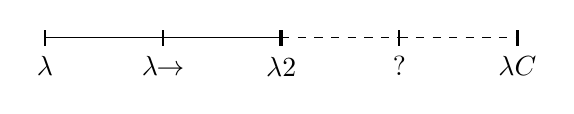
\begin{tikzpicture}
  \draw [-] (0,0) -- (1.5,0);
  \draw [-] (1.5,0) -- (3,0);
  \draw [dashed] (3,0) -- (4.5,0);
  \draw [dashed] (4.5,0) -- (6,0);
  \draw [thick] (0,-.1) node[below]{\(\lambda\)} -- (0,0.1);
  \draw [thick] (1.5,-.1) node[below]{\(\lambda\!\!\rightarrow\)} -- (1.5,0.1);
  \draw [ultra thick] (3,-.1) node[below]{\(\lambda 2\)} -- (3,0.1);
  \draw [thick] (4.5,-.1) node[below]{?} -- (4.5,0.1);
  \draw [thick] (6,-.1) node[below]{\(\lambda C\)} -- (6,0.1);
\end{tikzpicture}
\begin{flushleft}
  \textbf{Pros}: \textit{terms depending on types} (\(\Pi\)types)
  \par
  \textbf{Cons}: Lacks other dependencies
\end{flushleft}
The second-order lambda calculus \((\lambda2\)) derives its namesake from the
manner in which it extends \(\lambda\!\!\rightarrow\). \(\lambda 2\) categorizes
its expressions on \textit{two levels}: terms making up the first level and types
the second. In Type Theory, there are \textit{four levels}. We describe the four
levels in the section on \(\lambda\underline\omega\) (Section 4).

\(\lambda 2\) focuses on the addition of \textit{\(\Pi\)types}. \(\Pi\)types can
be thought of as a way of accurately representing \textit{dependencies} between
types and terms. In a sense, the same idea is encapsulated with arrow types but is
only used when the given dependency does not refer to \textit{terms depending on terms}.

In fact, \textit{terms depending on terms} are already present in \(\lambda\!\!\rightarrow\)
and \(\lambda\) when defining abstractions. The terms \(\lambda x\,.\,N\) and
\(\lambda x:\alpha\,.\,N : \alpha\rightarrow\gamma\) for \(\lambda\) and
\(\lambda\!\!\rightarrow\), respectively, are examples of terms depending on terms,
which in both cases is \(N\) depending on \(x\).

Since \(\lambda2\) is an extension of \(\lambda\!\!\rightarrow\), we must
define the \textit{type of all types} before \(\Pi\)types can be added, since
\(\lambda\!\!\rightarrow\) requires that everything be typed. Here we use the asterisk symbol,
\(*\), to represent the type of all types. Thus, all type variables
(\(\alpha,\beta,\gamma ...\)) are of type \(*\).

Adding \textit{terms depending on types} to \(\lambda\!\!\rightarrow\) raises the level
of expressivity and results in the system \(\lambda 2\). To show what specifically
has been added and also, consequently, what a \textit{term depending on a type} looks like,
we present the following example below.
\begin{itemize}
\item In \(\lambda\), the \textit{identity} function is \(\lambda x\,.\,x\), which functions
  for all possible inputs (e.g. Naturals, Integers, Booleans)
\item In \(\lambda\!\!\rightarrow\), there are too many identity functions
  (one for each simple type), when there should only be one.
\item To fix this, a \textit{polymorphic} identity function is made possible with
  \(\lambda2\). A function is \textit{polymorphic} when it generalizes over types
  (i.e., it can be applied to terms of different types). 
\item The polymorphic identity function is \(\lambda\,\alpha\,:\,*\,.\,\lambda\,x\,:\,\alpha\,.\,x\)
\end{itemize}
This particular polymorphic identity function can effectively serve as \textit{the}
identity function for all possible inputs \cite{gir}. For example, the function application
\((\lambda\alpha:*\,.\,\lambda x:\alpha\,.\,x) nat\) serves as the identity function
for Naturals since it \(\beta\)-reduces to \(\lambda x:nat\,.\,x\).

Typing the polymorphic identity function requires a \(\Pi\)type. This is necessary
because all polymorphic functions represent a form of dependency, and thus their
types should do the same. Hence, the most appropriate type for the polymorphic identity
function is \(\Pi\alpha:*\,.\,\alpha\rightarrow\alpha\).

From this we can see that the notion of types has been extended with a new type:
\(\Pi\)type. With \(\Pi\)types, the notion of \textit{simple types} has been removed
and the new definition for \textit{types} \((T)\) is:
\begin{itemize}
\item \((V_T)\) Type variable \((\alpha,\beta,\gamma\,...)\)
\item Arrow Type \((T\,\rightarrow\,T)\)
\item \(\Pi\)type \((\Pi V_T:*\,.\,T)\)
\end{itemize}
Consequently, the definition for \(\Lambda\)-terms \((\Lambda)\) has also changed.
The new definition for \(\Lambda\)-terms \cite{gir2}, which now includes dependent
terms, is given below.
\begin{itemize}
\item \((V)\) Term variable \((x,y,z...)\)
\item \((L)\) Abstraction \((\lambda V:T\,.\,\Lambda)\)
\item Application \((\Lambda_0\,\Lambda_1)\)
\item \((L_\Pi)\) Universal Abstraction \((\lambda V_T:*\,.\,\Lambda)\)
\item Universal Application \((L_\Pi\,T)\)
\end{itemize}
Having two instances of abstraction and application seems a bit excessive, however,
with what is explained later, the two variations are essentially equivalent if
we treat arrow types as \textit{special cases} of \(\Pi\)types.

Even with the addition of \(\Pi\)types and the expressivity that they bring,
\(\lambda2\) retains the strongly normalizing attribute of \(\lambda\!\!\!\rightarrow\).
From here, we may add different notions of type and term dependency until we reach
the full expressivity of \(\lambda C\).
%% \(\lambda2\), however, still does not have enough expressivity to function as an
%% effective foundation for logic or mathematics. It is still missing different notions
%% of type and term dependency.

%% TO DO: Fix beginning to state that we are adding \(\lambda\underline\omega\)
%% to lambda 2, resulting in \(\lambda\omega\). Mention that in this section
%% we are essentially describing the extension, not the system as a whole, since
%% that system is simply a combination of the two, nothing more. Don't forget
%% to mention System Fw

%% Also, fix the ending to make a transition into Lambda P.
\section*{4. Higher-Order (\(\lambda\underline\omega\))}
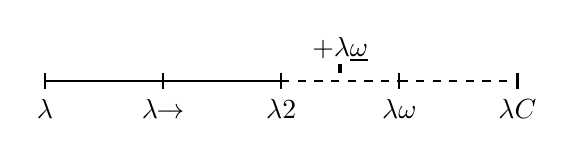
\begin{tikzpicture}
  \draw [-] (0,0) -- (1.5,0);
  \draw [-] (1.5,0) -- (3,0);
  \draw [dashed] (3,0) -- (4.5,0);
  \draw [dashed] (4.5,0) -- (6,0);
  \draw [thick] (0,-.1) node[below]{\(\lambda\)} -- (0,0.1);
  \draw [thick] (1.5,-.1) node[below]{\(\lambda\!\!\rightarrow\)} -- (1.5,0.1);
  \draw [thick] (3,-.1) node[below]{\(\lambda 2\)} -- (3,0.1);
  \draw [ultra thick] (3.75,0.1) node[above]{\(+\lambda\underline\omega\)} -- (3.75,0.21);
  \draw [thick] (4.5,-.1) node[below]{\(\lambda\omega\)} -- (4.5,0.1);
  \draw [thick] (6,-.1) node[below]{\(\lambda C\)} -- (6,0.1);
\end{tikzpicture}
\begin{flushleft}
  \textbf{Pros}: \textit{types depending on types}
  \par  
  \textbf{Cons}: No \(\Pi\)types
\end{flushleft}
Another name for \(\lambda\underline\omega\) is the
\textit{higher order \(\lambda\)-calculus} \cite{gir}. This system,
when combined with \(\lambda 2\) results in the system \(F_\omega\) or,
as notated above, \(\lambda\omega\). In this section, we primarily
describe the smaller \(\lambda\underline\omega\), an extension
from \(\lambda\!\!\rightarrow\), and not the combination.

\(\lambda\underline\omega\) adds a powerful construct to \(\lambda\!\!\rightarrow\):
\textit{type constructors}. In popular dependently typed programming languages
(e.g. Idris, Epigram, Agda), a common example of a type constructor is \textit{List}.
In these languages, to instantiate an object of type \textit{List} requires an
additional type. This additional type functions as the type of the instantiated list.
It is clear here that \textit{List} also has a type, namely \(*\rightarrow *\). As
an example, when the type constructor \textit{List} is given the type \(\sigma\),
it returns a list of type \(\sigma\) (i.e., \(List_\sigma\) or (List \(\sigma\))).
\textit{Type constructors} are thus functions that return types.

Similar to the requirements of adding \(\Pi\)types in \(\lambda2\), to add the
notion of \textit{types depending on types} in \(\lambda\underline\omega\), the
resulting expressions must be properly typed. For this, we add the notion
of \textit{kinds} \((K)\). A kind is one of:
\begin{itemize}
\item \(*\)
\item \(K\rightarrow K\)
\end{itemize}
Thus, all type constructors can be typed using a kind. Consequently, kinds must
also be typed, and all kinds have the type \(\square\) (e.g. \(*\), \(*\rightarrow *\),
\((*\rightarrow *)\rightarrow *\) are of type \(\square\)).

It is now appropriate to introduce the \textit{four levels} of Type Theory and
explain the relationship that the levels have with each other. The four levels are:
\begin{enumerate}
\item Terms only (specifically \(\Lambda\)-terms)
\item Types and type constructors
\item Kinds only
\item \(\square\) only
\end{enumerate}
The relationship between the levels is somewhat subtle while at the same time
intuitive. All expressions can be typed by an expression of the following level.
Grasping the relationship between the levels is important for understanding
the derivation rules of \(\lambda\underline\omega\), \(\lambda P\) (Section 5)
and \(\lambda C\) (Section 6), since most of the key premises of their rules include
\textit{sorts}. A sort (\(s\)) is one of:
\begin{itemize}
\item \(*\)
\item \(\square\)
\end{itemize}
In general, a sort is used to type \textit{types} and the type of types, \(*\),
a requirement of \(\lambda\!\!\rightarrow\). It is also a key aspect in determining,
at any given point in a \textit{derivation}, which two levels we are working in.
To clarify, the following example details how the \((conv)\) rule of
\(\lambda\underline\omega\) relates with the \textit{\(\beta\)-equivalence of types}:
\begin{itemize}
\item Take the type constructor \(\lambda\alpha :*\,.\,\alpha\rightarrow\alpha\,:\,*\rightarrow *\).
\item This constructor requires a type of type \(*\), so any arbitrary type (say \(\gamma\)) works.
\item Then, \((\lambda\alpha :*\,.\,\alpha\rightarrow\alpha)\)\(\gamma\) is a type.
\item Let \(A : (\lambda\alpha :*\,.\,\alpha\rightarrow\alpha)\gamma\).
\item Intuitively, we would want to be able to \textit{reduce} this to say that \(A : \gamma\rightarrow\gamma\).
\end{itemize}
Enabling the last point above requires \textit{type convertibility}. This notion is
captured by the \((conv)\) rule given below.
\begin{center}
  \infer[{if B =_\beta B' \quad (conv)}]
        {\Gamma\vdash\,A\,:\,B'}
        {\Gamma\vdash\, A\,:\,B & \Gamma\vdash\, B'\,:\,s}
\end{center}
We can read the above rule as follows: \(A\) can be of type \(B\) and \(B'\) if
\(B'\) is a sort, with a side condition that \(B =_\beta B'\). Depending on the value
of the sort, \(s\), we can determine whether \(A\), \(B\) and \(B'\) are terms or types.
For example, if \(s\) is \(*\), then \(B\) and \(B'\) are types and \(A\) must be a term.
Similarly, if \(s\) is \(\square\), then \(B\) and \(B'\) are kinds and \(A\)  must be a type.
Since \(\lambda\underline\omega\) can have applications of type constructors in its
type expressions and all legal applications must have \(\beta\)-reductions, we use
type convertibility rather often.

Thus, \(\lambda\underline\omega\) adds type constructors to \(\lambda\!\!\rightarrow\),
but it no longer has the expressivity of \(\Pi\)types. Extending \(\lambda\underline\omega\)
with \(\Pi\)types, however, is simple and is thus often done in the creation of
\textit{hybrid} systems, an example of which is \(\lambda\omega\) (\(\lambda 2\) +
\(\lambda\underline\omega\)). From here, we are only missing one form of term
and type dependency (i.e., \textit{types depending on terms}) before we reach the
expressivity of \(\lambda C\). We take the time to describe this dependency and
extension in the following section.

%% Doing so results in an entirely different system called
%% \(\lambda\omega\) (without the underscore) or \(F\omega\) \cite{gir}.There is only
%% one kind of dependency left, namely that of \textit{types depending on terms}, which
%% is added in \(\lambda P\).

%% TO DO: Fix introduction. Explain that we are essentially in a ``crossroads'' between
%% the above system and Lambda C. Once we add the extension describe in this section,
%% then we reach Lambda C. Keep the fact that this is a system that pays an integeral
%% role for making up Lambda C
\section*{5. Predicate Lambda Calculus (\(\lambda P\))}
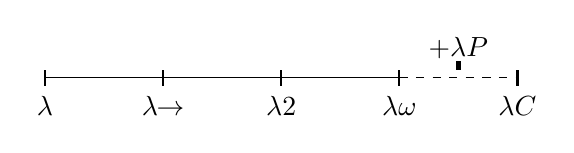
\begin{tikzpicture}
  \draw [-] (0,0) -- (1.5,0);
  \draw [-] (1.5,0) -- (3,0);
  \draw [-] (3,0) -- (4.5,0);
  \draw [dashed] (4.5,0) -- (6,0);
  \draw [thick] (0,-.1) node[below]{\(\lambda\)} -- (0,0.1);
  \draw [thick] (1.5,-.1) node[below]{\(\lambda\!\!\rightarrow\)} -- (1.5,0.1);
  \draw [thick] (3,-.1) node[below]{\(\lambda 2\)} -- (3,0.1);
  \draw [thick] (4.5,-.1) node[below]{\(\lambda\omega\)} -- (4.5,0.1);
  \draw [ultra thick] (5.25,0.1) node[above]{\(+\lambda P\)} -- (5.25,0.21);
  \draw [thick] (6,-.1) node[below]{\(\lambda C\)} -- (6,0.1);
\end{tikzpicture}
\begin{flushleft}
  \textbf{Pros}: \textit{types depending on terms}
  \par  
  \textbf{Cons}: Cannot encode \(\exists,\,\,\neg,\,\,\wedge,\,\, \text{and} \,\, \vee\)
\end{flushleft}
In this section, we set out to explain the final component of \(\lambda C\), namely
\(\lambda P\). \(\lambda P\) gives us \textit{types depending on terms}.

Out of all the components of \(\lambda C\) (Section 6), \(\lambda P\) plays one of
the more important roles in allowing \(\lambda C\) to serve as a possible foundation
for logic and mathematics. This is because \(\lambda P\) adds \textit{types depending on terms}
enabling it to encode \textit{minimal predicate logic} (described below), hence the
name \(\lambda P\). For our purposes, the overview of \(\lambda P\) describes how it does
this and why it is important.

\(\lambda P\) adds the notion of \textit{propositions} and \textit{predicates over types}.
To describe these entities and show what they look like in \(\lambda P\), the following example
details the type theoretic equivalent of the logical term:
\begin{center}
  \begin{tabu} {  X[c] | X[c] || X[c]  }
    \textbf{Inhabitants} & \textbf{Types} & \textbf{\(\lambda P\)} \\[0.05cm]
    \hline
    terms  & types & \(e : \alpha\) \\[0.05cm]
    \hline
    proofs & propositions & \(e : \rho\) \\[0.05cm]
  \end{tabu}\par\smallskip
  \textbf{Table 1:} PAT Interpretation
\end{center}
These entities correspond to the \textit{PAT-interpretation} of logic, a fundamental
aspect of Type Theory. PAT stands for \textit{propositions as types} and also
\textit{proofs as terms} \cite{how}. Together, they explain the correspondence between
\textit{Intuitionistic propositional logic} and Type Theory \cite{lof}.

In the more familiar Classical logic, every term can be evaluated to true or false.
In Intuitionistic Logic, the notion of truth corresponds to \textit{provability}.
Thus the ``truth'' of an expression \(B\) is determined by whether or not it can be proven
in a given context. In Type Theory, we represent this with the notion of \textit{inhabitation}.

We are already familiar with the notion of inhabitation, since the expression \(e : \rho\) can
also be read as \textit{the term e inhabits the type \(\rho\)} or \textit{e proves \(\rho\)}.
Returning to the idea of propositions as types, it is then clear why propositions \textit{are}
types, since they can be proven (\textit{inhabited}) by terms (proofs as terms).

Putting this all together, predicates then encapsulate the notion of
\textit{types depending on terms} in \(\lambda P\). For clarification, we give the
following example \cite{rng}:
\begin{itemize}
\item A predicate is of type \(\sigma\rightarrow *\), since it maps over an arbitrary type
  (here \(\sigma\)) and returns a proposition, which is a type \((*)\).
\item Let \(\rho_n\) be the proposition that \textit{n is a prime number}.
\item Propositions are sometimes notated as \(P(n)\). This notation states that the term
  \(n\) is allowed to appear \textit{free} in the term \(P\).
\item This notation is commonly mistaken for function invocation, so, for clarity, we use \(\rho_n\).
\item Then, \(\lambda n : nat\,.\,\rho_n\) is a predicate. Here, the type \(\rho_n\) depends
  on the value of the term \(n\).
\end{itemize}
Passing a Natural (say \(x\)) into \(\lambda n : nat\,.\,\rho_n\) would then return the
proposition \((\rho_x)\) that \(x\) is a prime number, which is only proven if an inhabitant
of type \(\rho_x\) can be found.

It is now appropriate to show the type theoretic encoding for \(\Rightarrow\) and \(\forall\),
which are the only connectives available in minimal predicate logic.%%  Below are the corresponding
%% \(\lambda P\) derivation rules that accurately model the behavior of the logical connectives of
%% minimal predicate logic.
\begin{center}
  \begin{tabu} {  X[c] | X[c]  }
  %% \begin{tabular}{ m{2.5cm} | m{2.5cm}  } 
    \textbf{Logic} & \textbf{Type Theory} \\[0.05cm]
    \hline
    \(\Rightarrow\)  & \(\rightarrow\)  \\[0.05cm]
    \hline
    \(A\Rightarrow B\)  & \(A\rightarrow B\)  \\[0.05cm]
    \hline
    \(\Rightarrow\)-intro  & \((abst)\)  \\[0.05cm]
    \hline
    \(\Rightarrow\)-elim  & \((app)\)  \\[0.05cm]
    \hline
    \hline
    \(\forall\)  & \(\Pi\)  \\[0.05cm]
    \hline
    \(\forall_ {x:\alpha} (\rho_x)\)  & \(\Pi x : \alpha\,.\,\rho_x\) \\[0.05cm]
    \hline
    \(\forall\)-intro  & \((abst)\)  \\[0.05cm]
    \hline
    \(\forall\)-elim  & \((app)\)  \\[0.05cm]
  \end{tabu}\par\smallskip
  \textbf{Table 2:} Type Theory \& Logic Correspondence
\end{center}
It seems strange that both the logical \textit{intro} and \textit{elim} rules for
\(\Rightarrow\) and \(\forall\) are modeled by the same derivation rule but are not
modeled by the same type theoretic connective. Returning to what we have mentioned in
the section for \(\lambda\underline\omega\), \(\lambda P\) treats \(\Pi\)types as a
special case for arrow types. Since \(\lambda P\) does not have the dependencies
mentioned in \(\lambda\underline\omega\) and \(\lambda 2\), it only needs to worry
about \textit{types depending on terms}. Clearly, \(\Pi\)types are \textit{only}
used when there is a dependency involved, which in \(\lambda P\) is present in terms
resembling \textit{predicates}. In arrow types, and consequently \(\Rightarrow\), the
expression to the right of \(\rightarrow\) can be thought of as \textit{independent}
from the expression on the left. To clarify this, the following example is given:
\begin{itemize}
\item \(\lambda x:\alpha\,.\,N\) can be modeled by an arrow type if \(x\)
  does not appear free in \(N\).
\item \(\lambda x:\alpha\,.\,\rho_x\) can only be modeled by a \(\Pi\)type since
  the term \(\rho_x\) depends on \(x\).
\end{itemize}
\(\lambda P\), however, has only one derivation rule for each \((abst)\) and \((app)\)
and the abstractions in these rules are always typed with a \(\Pi\)type. This means
that \(\Pi\)types can effectively model arrow types, since they hold more
information than \(\rightarrow\).

With the addition of \(\lambda P\), we have now seen all the various dependencies between
types and terms and the interesting constructs that they bring. We can now remove
the \textit{Cons} of all previously mentioned calculi by combining \(\lambda\!\!\rightarrow\),
\(\lambda 2\), \(\lambda\underline\omega\), and \(\lambda P\), resulting in \(\lambda C\).

\section*{6. Calculus of Constructions (\(\lambda C\))}
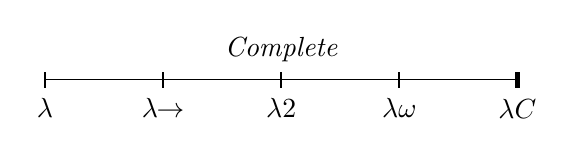
\begin{tikzpicture}
  \draw [-] (0,0) -- (1.5,0);
  \draw [-] (1.5,0) -- (3,0);
  \draw [-] (3,0) -- (4.5,0);
  \draw [-] (4.5,0) -- (6,0);
  \draw [thick] (0,-.1) node[below]{\(\lambda\)} -- (0,0.1);
  \draw [thick] (1.5,-.1) node[below]{\(\lambda\!\!\rightarrow\)} -- (1.5,0.1);
  \draw [thick] (3,-.1) node[below]{\(\lambda 2\)} -- (3,0.1);
  \draw [thick] (3,0.1) node[above]{\em Complete} -- (3,0.1);
  \draw [thick] (4.5,-.1) node[below]{\(\lambda\omega\)} -- (4.5,0.1);
  \draw [ultra thick] (6,-.1) node[below]{\(\lambda C\)} -- (6,0.1);
\end{tikzpicture}
\begin{flushleft}
  \textbf{Pros}: Able to fully encode \textit{Constructive Logic}
  \par  
  \textbf{Cons}: ?
\end{flushleft}
The Calculus of Constructions (\(\lambda C\)) is the culmination of the \(\lambda\)-calculi
we have mentioned and described. It retains the strongly normalizing attribute of
its components and their various forms of type and term dependency. With this power,
\(\lambda C\) can effectively serve as a foundation for logic and mathematics and
as well a \textit{typed programming language}.

The figure below is Barendregt's \(\lambda\)-cube \cite{bar2} and notates the
relationship between the calculi we mentioned earlier. The base of the cube
starts with \(\lambda\!\!\rightarrow\). From there, extending upwards results in
\(\lambda 2\), extending to a third dimension results in \(\lambda\underline\omega\),
and extending rightwards results in \(\lambda P\). From these other points, it is
also possible to extend to other calculi in the same manner. For example, \(\lambda P\)
can be extended with either \(\lambda2\) or \(\lambda\underline\omega\),
resulting in \(\lambda P2\) or \(\lambda P\underline\omega\) respectively.
This means that there actually are multiple ways to reach \(\lambda C\) from
\(\lambda\!\!\rightarrow\). Here, we first extended \(\lambda\!\!\rightarrow\)
first with \(\lambda2\), then added \(\lambda\underline\omega\) to reach
\(\lambda\omega\), then added \(\lambda P\) to reach \(\lambda C\). Looking again
at the cube, this leaves \(\lambda C\) in the position of the cube that
encompasses \textit{all} possible extensions from \(\lambda\!\!\rightarrow\).
\begin{center}
  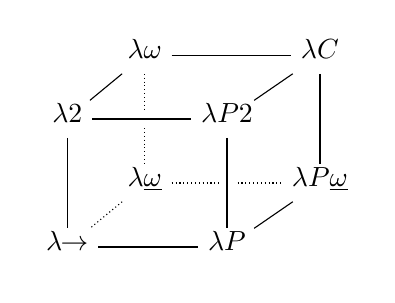
\begin{tikzpicture}[
      back line/.style={densely dotted},
      cross line/.style={preaction={draw=white, -,
          line width=6pt}}]
    \matrix (m) [matrix of math nodes,
      row sep=1em, column sep=.75em,
      text height=1ex,
      text depth=0.5ex]{
      & \lambda\omega & & \lambda C \\
      \lambda 2 & & \lambda P2 \\
      & \lambda\underline\omega & & \lambda P\underline\omega \\
      \lambda\!\!\rightarrow  & & \lambda P \\
    };
    \path[-]
    (m-1-2) edge (m-1-4)
    edge (m-2-1)
    edge [back line] (m-3-2)
    (m-1-4) edge (m-3-4)
    edge (m-2-3)
    (m-2-1) edge [cross line] (m-2-3)
    edge (m-4-1)
    (m-3-2) edge [back line] (m-3-4)
    edge [back line] (m-4-1)
    (m-4-1) edge (m-4-3)
    (m-3-4) edge (m-4-3)
    (m-2-3) edge [cross line] (m-4-3);
  \end{tikzpicture}
\end{center}

\(\lambda C\) derives its name from Constructive Logic by its creator Thierry Coquand \cite{coq1}.
\(\lambda C\) is the \textit{only} \(\lambda\)-calculus that can fully encode the
logical connectives (\(C\)) of Intuitionistic Logic. It does this by combining
different forms of type and term dependencies from its components. The type of
these encodings are given below.
\begin{center}
  \begin{tabular}{ m{0.3cm} | m{7.4cm}  } 
    \textbf{C} & \textbf{\(\lambda C\) Type} \\[0.1cm]
    \hline      
    \(\perp\)  & \(\Pi\alpha : *\,.\,\alpha\)  \\[0.1cm]
    \hline
    \(\neg\)  & \(\lambda\alpha : *\,.\,(\alpha\rightarrow\perp)\)  \\[0.1cm]
    \hline
    \(\Rightarrow\)  & \(\lambda\alpha : *\,.\,\lambda\beta : *\,.\,\alpha\rightarrow\beta\)  \\[0.1cm]
    \hline
    \(\wedge\)  & \(\lambda\alpha : *\,.\,\lambda\beta : *\,.\,\Pi\gamma : *\,.\,(\alpha\rightarrow\beta\rightarrow\gamma)\rightarrow\gamma\)  \\[0.1cm]
    \hline
    \(\vee\)  & \(\lambda\alpha : *\,.\,\lambda\beta : *\,.\,\Pi\gamma : *\,.\,(\alpha\rightarrow\gamma)\rightarrow(\beta\rightarrow\gamma)\rightarrow\gamma\)  \\[0.1cm]
    \hline
    \(\forall\)  & \(\lambda\sigma : *\,.\,\lambda\rho : \sigma\rightarrow *\,.\,\Pi x : \sigma\,.\,\rho_x\)  \\[0.1cm]
    \hline
    \(\exists\)  & \(\lambda\sigma :*\,.\,\lambda\rho : \sigma\rightarrow *\,.\,\Pi\alpha : *\,.\,((\Pi x : \sigma\,.\,(\rho_x\rightarrow\alpha))\rightarrow\alpha\)  \\[0.1cm]
  \end{tabular}\par\smallskip
  \textbf{Table 3:} Connective Encodings
\end{center}
The types of these connectives are type constructors that return propositions
(types). Some of these type constructors can be encoded by a smaller subset
of \(\lambda C\) (i.e., \(\perp\) can be encoded by \(\lambda 2\)),
but some require a larger combination (i.e., \(\exists\) can only be encoded by
\(\lambda C\)). Below is a table containing the necessary system to encode each logical connective.
\begin{center}
  \begin{tabu} {  X[c] | X[c]  }
    \textbf{Connective} & \textbf{System Required} \\[0.05cm]
    \hline
    \(\perp\)  & \(\lambda2\)  \\[0.05cm]
    \hline
    \(\neg\)  &  \(\lambda\omega\) \\[0.05cm]
    \hline
    \(\Rightarrow\)  &  \(\lambda2\) or \(\lambda\underline\omega\) \\[0.05cm]
    \hline
    \(\wedge\)  &  \(\lambda\omega\) \\[0.05cm]
    \hline
    \(\vee\)  &   \(\lambda\omega\) \\[0.05cm]
    \hline
    \(\forall\)  & \(\lambda P2\) or \(\lambda P\underline\omega\) \\[0.05cm]
    \hline
    \(\exists\)  & \(\lambda C\)  \\[0.05cm]
  \end{tabu}\par\smallskip
  \textbf{Table 4:} System Requirements
\end{center}
The simplest way to explain how these encodings accurately model their respective
connective is to show how they are \textit{introduced} and \textit{eliminated}.
In \(\lambda C\), this is done solely by \((abst)\) and \((app)\), respectively.
Thus, the rules mentioned in the following sections are special cases of \((abst)\)
and \((app)\) modeled specfically for their respective connectives.

\subsubsection* {Negation (\(\neg\)) and Absurdity (\(\perp\))}
We describe \(\neg\) and \(\perp\) together because they are most commonly used
for one purpose: \textit{ex falso}. \textit{Ex falso} is a logical term that means
``from absurdity comes anything one wants.'' In Type Theory, this is equivalent to
``if \(\perp\) is inhabited, then everything is inhabited''. This behavior is modeled
by \(\perp\!\!-elim\). To find an inhabitant of \(\perp\), we must first derive a term
of type \(\perp\) via \(\perp\!\!-intro\). Both of these rules are given below.
\begin{center}
  \begin{tabu}{ X[c]  X[c] }
    \infer[{(\perp\!\! -intro)}]{NM:\,\perp}{M:A & N:A \rightarrow\perp} &
    \infer[{(\perp\!\! -elim)}]{NA:A}{N:\,\perp}  \\
  \end{tabu}
\end{center}
The type theoretic reading for \(\perp\!\! -intro\) is
\textit{if we can derive a term of type A and a term of type \(A\rightarrow\perp\), we can derive \(\perp\)}.
For clarification, the example below shows how these rules are used in a general
type theoretic setting.
\begin{itemize}
\item Assume that \(m\) is of type \(A\)
\item Assume that \(n\) is of type \(\neg A\)
\item By definition, \(n\) is also of type \(A\rightarrow\perp\)
\item Then, \(n\,m : \,\perp\)
\item Say we want to inhabit the type \(\gamma\)
\item From the type of \(\perp\), \(n\,m\) is also of type \(\Pi\alpha:*\,.\,\alpha\)
\item Then, \(n\,m\,\gamma : \gamma\) (i.e. \(n\,m\,\gamma\) proves \(\gamma\))
\end{itemize}

\subsubsection* {Implication (\(\Rightarrow\))}
There is a rather clear one-to-one correspondence between \(\Rightarrow\) and \(\rightarrow\).
The encoding for \(\Rightarrow\) we mentioned earlier is simply the polymorphic version,
as are all others the others in Table 3. This means that it takes two types and
creates an arrow type that maps the first type into the second. Like \(\lambda P\),
the arrow type of \(\lambda C\) is actually a \(\Pi\)type, so \((abst)\) and \((app)\)
are sufficient enough to model the proper behavior of \(\Rightarrow\).

\subsubsection* {Conjunction (\(\wedge\)) and Disjunction (\(\vee\))}
The encodings for \(\wedge\) and \(\vee\) correspond to their \textit{second-order encodings}.
The second order encoding is necessary, because the first order encoding is only
compatible with Classical logic. Since Intuitionistic logic is essentially a
\textit{subset} of Classical logic, its rules must be more general \cite{lof}.
In a simple example, conjunction corresponds to a typed \textit{pair} and
disjunction corresponds to a \textit{disjoint union}.
\begin{itemize}
\item Assume \(x:\alpha\), \(y:\beta\)
\item Assume \(z\) is a pair comprised of \(x\) and \(y\)
\item Then, \(z:(\alpha\times\beta)\), respresenting a conjunction of \(x\) and \(y\).
  Here, we can deconstruct \(z\) and get \(x:\alpha\) and \(y:\beta\).
\item For disjunction, deconstructing an expression of type \((\alpha + \beta)\)
  requires \textit{case analysis} or pattern matching. When we deconstruct
  such a term, we get either a term of type \(\alpha\) or a term of type \(\beta\).
\end{itemize}

%% Hence,
%% the encodings in \(\lambda C\) must model the more general versions of the \(\wedge\)
%% and \(\vee\) rules of Intuitionistic logic, included below.
%% \begin{center}
%%   \begin{tabu}{ X[c] }
%%     \infer[{(\wedge\!\! -\!intro)}]{\Pi C:*\,.\,(A\rightarrow B\rightarrow C)\rightarrow C}{A & B} \\
%%     \infer[{(\wedge\!\! -\!elim_1)}]{A}{\Pi C:*\,.\,(A\rightarrow B\rightarrow C)\rightarrow C} \\
%%     \infer[{(\wedge\!\! -\!elim_2)}]{B}{\Pi C:*\,.\,(A\rightarrow B\rightarrow C)\rightarrow C} \\
%%     \infer[{(\vee\!\! -\!intro_1)}]{\Pi C:*\,.\,(A\rightarrow C)\rightarrow(B\rightarrow C)\rightarrow C}{A} \\
%%     \infer[{(\vee\!\! -\!intro_2)}]{\Pi C:*\,.\,(A\rightarrow C)\rightarrow(B\rightarrow C)\rightarrow C}{B} \\
%%     \infer[{{\footnotesize (\vee\!\! -\!elim\!)}}]{C}{\Pi C:*\,.\,(A\rightarrow C)\rightarrow(B\rightarrow C)\rightarrow C & A\rightarrow C & B\rightarrow C} \\
%%   \end{tabu}
%% \end{center}
\subsubsection* {Quantifiers (\(\forall\) and \(\exists\))}
Similar to \(\Rightarrow\) and \(\rightarrow\), \(\forall\) is modeled accurately by
\(\Pi\). Like \(\lambda P\), the \((abst)\) and \((app)\) rules of \(\lambda C\) are
already perfect models for the rules of \(\forall\).

\(\exists\), however, is quite a bit more complicated. To clarify, the following
example details \(\exists\!\!-\!\!elim\) rule.
\begin{itemize}
\item Assume \(\sigma:*\),\(\,\,\rho:\sigma\rightarrow *\), and \(A:*\)
\item Assume \(y:\Pi\alpha:*\,.\,((\Pi x:\sigma\,.\,(\rho_x\rightarrow\alpha))\rightarrow\alpha)\)
\item Assume \(z:\Pi x:\sigma\,.\,(\rho_x\rightarrow A)\)
\item Then, \(y\,A:(\Pi x:\sigma\,.\,(\rho_x\rightarrow A))\rightarrow A)\)
\item \(y\,A\) is an abstraction: \(\lambda u:(\Pi x:\sigma\,.\,(\rho_x\rightarrow A))\,.\,A\)
\item Then, \(y\,A\,z:A\)
\end{itemize}
In the above example, \textit{y} is an encoding of the existential quantifier,
\(\exists\), and \(z\) is an encoding for the universal quantifier, \(\forall\).
To derive \(y\), we use \(\exists\!\!-\!\!intro\). To do so, we need a type,
a predicate over said type, an inhabitant of said type, and a proof of said predicate.
\begin{itemize}
\item Assume \(\sigma:*\),\(\,\,\rho:\sigma\rightarrow *\),\(\,\,a:\sigma\), and \(u:\rho_a\)
\item With these assumptions, we may simply abstract over \(a\) and \(u\) to
  create an inhabitant of \(\exists\).
\item Then, \(\lambda\alpha:*\,.\,\lambda v:(\Pi x:\sigma\,.\,(\rho_x\rightarrow\alpha))\,.\,v\,a\,u :\Pi\alpha:*\,.\,((\Pi x:\sigma\,.\,(\rho_x\rightarrow\alpha))\rightarrow\alpha)\)
\end{itemize}
This encoding of the existential quantifier is only possible in \(\lambda C\),
since it requires all forms of term and type dependency. This power and expressivity
found in \(\lambda C\) is the reason why it is commonly used as a foundation for
proof assistants. \(\lambda C\), however, is also commonly extended with
\textit{inductive} types, allowing it to prove properties on recursive data structures.

\subsubsection*{Inductive Constructions}
The extension of \(\lambda C\) with inductive types allows an encoding of recursive
data structures and functions, while retaining the strongly normalizing attribute of
\(\lambda\!\!\rightarrow\). This system is called the
\textit{Calculus of Inductive Constructions} \cite{bert}.

To show the power of this system, we present a proof of the \textit{double-reverse theorem}
in Idris. The double-reverse theorem states that the reverse of the reverse of
an arbitrary list, \(l\), is equal to \(l\). Below is the theorem we use for our proof.

{\small
\begin{verbatim}
drev_thm : (xs : List a) -> rev (rev xs) = xs
\end{verbatim}
}

In our type expressions, we exclude any implicit \(\Pi\)types that Idris can infer.
Specifically, we exclude the \(\Pi\)type {\small\tt \{a:Type\}}, since it is
clear in our type expressions that {\small\tt a} is a type.

To show the usage and general behavior of proof assistants, we use Idris'
\textit{interactive prover} to prove the double-reverse theorem. Here, the user is
prompted by a number of goals and assumptions in which the user is allowed to
interact with using a series of defined commands, called \textit{tactics}.
Afterwards, we show an equivalent proof using a more ``manual'' approach.

For our proof, we use the following definition of reverse:

{\small
\begin{verbatim}
rev : List a -> List a
rev [] = []
rev (x :: xs) = rev xs ++ [x]
\end{verbatim}}

To those familiar with the syntax of Haskell, this definition of {\small\tt rev}
is recursively defined for an arbitrary list ({\small\tt xs}), hence the need
for an \textit{inductive} proof. Since {\small\tt rev} is defined using
{\small\tt ++}, Idris' list append, it is helpful to first prove other properties
with respect to {\small\tt ++}. In this case, we need a proof for
\textit{the distributivity of} {\small\tt ++} \textit{over} {\small\tt rev},
which in turn requires a proof of {\small\tt ++}-\textit{identity} and the
\textit{associativity of} {\small\tt ++}.

{\small
\begin{verbatim}
rev_append_dist : (xs,ys : List a) -> 
    rev (xs ++ ys) = rev ys ++ rev xs
append_id : (xs : List a) -> xs ++ [] = xs
\end{verbatim}}

We provide these proofs in full after completing the double-reverse theorem.
Since Idris has {\small\tt appendAssociative}, we do not include a proof
of the associativity of {\small\tt ++}.

Now we are ready to start the interactive prover. To start, we must first
allow Idris to create a pattern-match statement for {\small\tt drev\_thm}.

{\small
\begin{verbatim}
drev_thm xs = ?drev_thm_rhs
\end{verbatim}
}

Here, {\small\tt ?drev\_thm\_rhs} represents an \textit{incomplete proof}.
We now have the option of completing the proof using the interactive prover.
The proof starts with no assumptions and a single goal.

{\small
\begin{verbatim}
{hole0} : (a : Type) -> (xs : List a) ->
   rev (rev xs) = xs
\end{verbatim}
}

The only valid tactic for this step is {\small\tt intros}, which creates a
new goal and moves all expressions to the left of an \(\rightarrow\) into the
proof's assumption list.

{\small
\begin{verbatim}
Assumptions: (a : Type), (xs : List a)
{hole2} : rev (rev xs) = xs
\end{verbatim}
}

From these assumptions, it is clear that {\small\tt xs} is a list. Knowing
this, the next valid tactic is {\small\tt induction xs}, allowing us to
perform induction on the list {\small\tt xs}. This command creates 2
subgoals: \textit{base} and \textit{induction}. Peforming induction on a list
reveals its \textit{constructors}, {\small\tt Nil} and {\small\tt (::)}
(i.e., empty list and \textit{cons}). By default, we must first prove the base
subgoal.

{\small
\begin{verbatim}
elim_Nil0 : rev (rev []) = []
\end{verbatim}
}

Idris can \textit{normalize} this goal using the {\small\tt compute} tactic,
resulting in {\small\tt [] = []}. Since this expression \textit{holds by reflexivity},
using the {\small\tt trivial} tactic completes base subgoal.

{\small
\begin{verbatim}
elim_::0 : (t__0 : a) -> (l__0 : List a) -> 
    (rev (rev l__0) = l__0) ->
    rev (rev (t__0 :: l__0)) = t__0 :: l__0
\end{verbatim}
}

The above expression is the start of the inductive subgoal, which gives us an
\textit{inductive hypothesis} ({\small\tt IH}). Here, we can use a specialized
{\small\tt intro} tactic to name to our inductive hypothesis and as well
as rename the variables {\small\tt t\_\_0} and {\tt l\_\_0}. Here, we
name our inductive hypothesis {\tt IH} and rename {\tt t\_\_0} and {\tt l\_\_0}
as {\tt y} and {\tt ys}, respectively.

{\small
\begin{verbatim}
Apply (intro y,ys,ih) =>
Assumptions: (a : Type), (xs : List a), (y : a), 
    (ys : List a), (IH : rev (rev ys) = ys)
{hole11} : rev (rev (y :: ys)) = y :: ys
\end{verbatim}
}

We normalize this subgoal using {\small\tt compute}.

{\small
\begin{verbatim}
{hole11} rev (rev ys ++ [y]) = y :: ys
\end{verbatim}
}

Next, we use the proof of {\small\tt rev\_append\_dist} on the lists
{\small\tt (rev ys)} and {\small\tt [y]}. To do this, we apply
{\small\tt rewrite sym (rev\_append\_dist (rev ys) [y])} to the above
subgoal. This simplifies {\small\tt rev (rev ys ++ [y])} with respect to
\textit{symmetry}.

{\small
\begin{verbatim}
{hole12} : y :: rev (rev ys) = y :: ys
\end{verbatim}
}

Now, we have a subgoal that we can rewrite using our inductive hypothesis
({\small\tt IH}), {\small\tt rev(rev ys) = ys}. We do this by using
{\small\tt rewrite sym IH}, resulting in another expression that holds by reflexivity.

{\small
\begin{verbatim}
{hole29} : y :: ys = y :: ys
\end{verbatim}
}

Applying {\small\tt trivial} finishes the proof. Using the {\small\tt qed}
tactic gives the option of saving our proof (i.e. our tactics). Below are the proofs
for {\small\tt append\_id}, {\small\tt rev\_append\_dist} and {\small\tt drev\_thm}.

{\small
\begin{verbatim}
drev_thm
    intros
    induction xs
    compute
    trivial
    intro y,ys,IH
    compute
    rewrite sym (rev_append_dist (rev ys) [y])
    rewrite sym IH
    trivial
rev_append_dist
    intros
    induction xs
    compute
    induction ys
    trivial
    intro z,zs,IH
    compute
    rewrite (append_id (rev zs ++ [z]))
    trivial
    intro z,zs,IH
    compute
    rewrite sym IH
    rewrite appendAssociative (rev ys) (rev zs) [z]
    trivial
append_id
    intros
    induction xs
    compute
    trivial
    intro y,ys,IH
    compute
    rewrite sym IH
    trivial
\end{verbatim}
}

Essentially, using the interactive prover allows us to construct inhabitants
for the types of our theorems. We may choose to do a similar proof using
only \textit{rewrite} rules. This makes our proofs more compact and gives
us the feeling of constructing them from the ground up in a more familiar
fashion. For example, the complete proof for {\small\tt drev\_thm} using
only {\small\tt rewrite} rules is given below.

{\small
\begin{verbatim}
1| drev_thm : (xs : List a) -> rev (rev xs) = xs
2| drev_thm [] = Refl
3| drev_thm (x :: xs) = 
     rewrite rev_append_dist (rev xs) [x] in
       rewrite drev_thm xs in Refl
\end{verbatim}
}

To generate this proof, we need a type to prove (viz. first line) and
pattern match expressions (viz. second and third line). Here, we use
two pattern match expressions, one for \textit{base} and \textit{inductive}.
From here, we have two incomplete proofs:

{\small
\begin{verbatim}
drev_thm : (xs : List a) -> rev (rev xs) = xs
drev_thm [] = ?drev_thm_rhs_1
drev_thm (x :: xs) = ?drev_thm_rhs_2
\end{verbatim}
}

Since our proof uses the propositional connective {\small\tt =}, we are
required to build up proofs on {\small\tt Refl}. Thus, we are finished
with a given proof only when the goal we are presented with is provable using
{\small\tt Refl} (i.e., the goal is of the form {\small\tt x = x}, for any
arbitrary expression {\small\tt x}.).

In this proof method, we are free to choose whichever case to prove first, since
in both cases the proofs are independent of each other. Here, we start with the
base case. The base case ({\small\tt ?drev\_thm\_rhs\_1}) gives us the goal:

{\small
\begin{verbatim}
`--          a : Type
-------------------------
drev_thm_rhs_1 : [] = []
\end{verbatim}
}

Since {\small\tt [] = []} is provable by {\small\tt Refl}, we write \((2)\) above.
The inductive case ({\small\tt ?drev\_thm\_rhs\_2}) requires a bit more work.

{\small
\begin{verbatim}
`--          a : Type
             x : a
            xs : List a
----------------------------------------------
drev_thm_rhs_2 : rev (rev xs ++ [x]) = x :: xs
\end{verbatim}
}

Here, the expression {\small\tt rev (rev xs ++ [x])} can be simplified using
a proof of {\small\tt rev\_append\_dist} on {\small\tt (rev xs)} and {\small\tt [x]},
resulting in the updated goal below.

{\small
\begin{verbatim}
`--          a : Type
             x : a
            xs : List a
 _rewrite_rule : rev [x] ++ rev (rev xs) = 
                   rev (rev xs ++ [x])
--------------------------------------------
drev_thm_rhs_2 : x :: rev (rev xs) = x :: xs
\end{verbatim}
}

{\small\tt \_rewrite\_rule} is the proof of {\small\tt rev\_append\_dist}
on the lists {\small\tt (rev xs)} and {\small\tt [x]}. From here, the only
valid step is to perform induction on {\small\tt xs}. In this proof method,
we perform induction and the rewriting of an inductive hypothesis with a
single {\small\tt rewrite} rule. We use {\small\tt rewrite drev\_thm xs}
giving us the assumption that {\small\tt xs = rev (rev xs)} holds,
resulting in the expression provable by {\small\tt Refl} given below.

{\small
\begin{verbatim}
`--          a : Type
             x : a
            xs : List a
 _rewrite_rule : rev [x] ++ rev (rev xs) = 
                  rev (rev xs ++ [x])
_rewrite_rule1 : xs = rev (rev xs)
------------------------------------------
drev_thm_rhs_2 : x :: xs = x :: xs
\end{verbatim}
}

We then write \((3)\) in the finished proof above for {\small\tt drev\_thm}.
For more examples using this proof method, we include the proofs of
{\small\tt rev\_append\_dist} and {\small\tt append\_id} below.
For clarity, we follow the same formatting used in the complete proof
of {\small\tt drev\_thm} (e.g. \((1)\) is the type statement,
\((2)\) is the proof of the base case, \((3)\) is the proof of the
inductive/recursive case).

{\small
\begin{verbatim}
1| append_id : (xs : List a) -> xs ++ [] = xs
2| append_id [] = Refl
3| append_id (x :: xs) = 
     rewrite append_id xs in Refl

1| rev_append_dist : (xs,ys : List a) -> 
     rev (xs ++ ys) = rev ys ++ rev xs
2| rev_append_dist [] ys = 
     rewrite append_id (rev ys) in Refl
3| rev_append_dist (x :: xs) ys = 
     rewrite rev_append_dist xs ys in 
       rewrite appendAssociative (rev ys) 
                                 (rev xs) 
                                 [x] in Refl
\end{verbatim}
}

In these proofs, the order that we apply {\small\tt rewrites} does not matter.
We can see the reason for this when we look at the final goal for
{\small\tt drev\_thm}. The expressions above the line are assumptions in
\textit{context}. Their order only matters when expressions are dependent of
each other. For example, the expression \mbox{{\small\tt (a : Type)}} must
come before {\small\tt (x : a)} and \mbox{{\small\tt (xs : List a)}} since
{\small\tt a} appears in these expressions and guarantees that {\small\tt a}
is a type. On the other hand, both {\small\tt rewrite} rules do not
\textit{introduce} any new names or expressions into context. Instead, they behave,
more or less, like proofs that allow us to construct new goals. This is
ideal since this maintains the correspondence between \textit{programs} and
\textit{proofs}. That is, in either case, the manner that we choose to (correctly)
evaluate or reduce them does not (and should not) affect the final outcome.

%%%% HoTT Route
Write a better segue.
%% From here, we are now familiar with handling inductive types, one of which is type of
%% \textit{equality}. Briefly, equality is built up with a single constructor, \textit{refl}.
%% Refl, or \textit{reflexivity}, states that an expression is only equal to itself, similar to
%% Liebniz's Law. We can see this in Idris' interactive prover when applying the tactic
%% {\small\tt trivial}, since this tactic attempts to reduce a goal with respect to reflexivity.
%% When \(\lambda C\) is extended with induction and the notion of equality, it is possible
%% to extend it even further to a system that simulates \textit{Homotopy Type Theory}. 

\subsection*{Homotopy Type Theory}
Equivalence is a proof of equality, or equivalence is equivalent to equality. Equality is
path equality (homotopical). Two types are equivalent, when they are equivalent with
respect to an existence between their elements.

%%%% Co-induction Route
%% \par\hspace{2ex}  
%% In a co-inductive system, we can only prove properties with respect to \textit{productivity} and \textit{bisimilarity}.
%% In other words, we can only prove properties on the behavior of infinite data by appealing to the manner in which they are built up.
%% \subsubsection*{Co-inductive Constructions}
%% Extending \(\lambda C\) with co-inductive types allows an encoding of infinite data structures (e.g. lazy lists or \textit{streams}),
%% resulting in the system of \textit{The Calculus of Co-inductive Constructions} \cite{unknown}.
%% \par\hspace{2ex}  
%% We, once again, use Idris to model a simple co-inductive proof. Since Idris is built on Haskell, it already has access to
%% streams \cite{unknown}. Unfortunately, Idris' interactive prover does not yet fully support co-inductive proofs,
%% however, we can still prove certain properties of infinite data by appealing to induction.

\section* {Final Remarks}
\begin{itemize}
\item Talk about \(\lambda C\) and \textit{why} it is a good foundation for
  learning and modelling Type Theory
\item Specifically, it can be taught in bits and pieces from its components,
  which comprise the majority of the ideas of type theory
\item Also, since Type theory is meant to be \textit{computable}, it should be
  modelled by something that can compute. \(\lambda C\) does this since it is a
  system built on computation (i.e., a calculus). Effectively, this gives rise to
  something that can be simulated by a computer program (i.e., all features of type
  theory can be prescribed an algorith, since it can be modelled entirely by \(\lambda C\)).
\item Briefly talk about HoTT and its relationship with Type theory and how it
  is essentially the new foundation for mathematics (maybe talk about how it supports
  both classical and constructive logic?)
\end{itemize}
%% The Calculus of Constructions is great system to start out with in learning Type Theory. It, however, should not be the stopping point.
%% In fact, there are already two variants of the calculus that are more powerful and expressive: the Calculus of Inductive Constructions
%% and the Calculus of Co-inductive Constructions. The former is the system that the proof assistant Coq is built on and is a requirement
%% to add \textit{recursion} and an encoding of \textit{peano} Natural numbers.
%% The later is a system that permits \textit{infinite data types} (i.e. lazy lists or \textit{streams}) and
%% has the fascinating ability to prove properties about them. Functional programming would not be
%% as expressive and powerful as it is today without these systems.
``Type Theory and Formal Proof'' offers insight on a variant of \(\lambda C\) called
\(\lambda D\). \(\lambda D\) is a system that has similar power to the Calculus of
Inductive Constructions by extending \(\lambda C\) with \textit{definitions}. In effect,
\(\lambda D\) retains the relative simplicity of the base \(\lambda C\) system,
while also simulating the power of the more complicated \(\lambda C\) variants.

Write a better final paragraph. Don't include opinion.
%% In this paper, we simply offer our own perspective of an ``introduction'' to Type Theory with hopes of inspiring
%% individuals to wade into the field. If they were to do so, we hope that they would find as much fascination and
%% intrigue as many of the forerunners of the field have found in it.
%%%%%%%%%%%%%%%%%%%%%%%%%%%%%%%%%%%%%%%
\begin{thebibliography}{1}
  %% HP Barendregt 1984
  %% HP Barendregt 1992
  %% Church 1940
  %% Thierry Coquand 1988
  %% Girard 1972
  %% Martin-Lof 1980
  %% Nederpelt and Geuvers 2014
  %% Sanchis

\bibitem{bar1} Henk Barendregt. {\em The Lambda Calculus: Its Syntax and Semantics}
  1984: Elsevier Science.

\bibitem{bar2} Henk Barendregt. {\em Lambda Calculi with types}
  1992: Handbook of Logic in Computer Science, pp. 117-309, Oxford University Press.

\bibitem{bert} Yves Bertot and Pierre Cast\'eran. {\em Interactive Theorem Proving and Program
  Development: Coq\'Art: the Calculus of Inductive Constructions} 2004: Springer.

\bibitem{church} Alonzo Church. {\em A formulation of the simple theory of types}
  1940: Journal of Symbolic Logic, 5, pp. 56-68.

\bibitem{coq1} Thierry Coquand and G\'erard Huet. {\em The Calculus of Constructions}
  1988: Information and Computation, 76, pp. 95-120.

\bibitem{gir} Jean-Yves Girard. {\em Interpr\'etation fonctionnelle et \'elimination des coupures de l’arithm\'etique d’ordre sup\'erieur}
  1972: PhD thesis, Universit\'e Paris VII.

\bibitem{gir2} Jean-Yves Girard, Yves Lafont, and Paul Taylor. {\em Proofs and Types}
  1989: Cambridge University Press, pp. 82-86.

\bibitem{how} William Howard. {\em The formulae-as-types notion of construction}
  1980: Seldin and Hindley, pp. 479-490.

\bibitem{lof} Per Martin-L\"of. {\em Intuitionistic Type Theory}
  1980: Bibliopolis

\bibitem{rng} Rob Nederpelt and Herman Geuvers. {\em Type Theory and Formal Proof}
  2014: Cambridge University Press.
  
\bibitem{san} Luis Sanchis. {\em Functionals defined by Recursion}
  1967: Notre Dame Journal of Formal Logic VIII, pp. 161-174.
  
\end{thebibliography}
%%%%%%%%%%%%%%%%%%%%%%%%%%%%%%%%%%%%%%%
\end{document}
